%The average daily, per-person rate of interactions involving data is expected to increase twentyfold by 2025, as everything becomes data-enabled and generates data\footnote{International Data Corporation, \href{https://www.seagate.com/files/www-content/our-story/trends/files/Seagate-WP-DataAge2025-March-2017.pdf}{Data Age 2025}, IDC Whitepaper}. 

%, on two main topics that are
%relevant for European economical advancement: automotive traffic\footnote{; The European Union, \href{https://europa.eu/european-union/about-eu/figures/economy_en}{Economy: Transport}, accessed online 12/2019} and IoT sensors$^8$. 

%\subsubsection{Originality, relevance and timeliness of the program}




%The ESRs involved in \acronym will work within the competitive world of 

%The sheer size of the datasets collected by scientific experiments is leading researchers in HEP towards advanced methods normally used in industry, such as ML and AI. 
%The advancement of our understanding of the basic building blocks of matter 
%requires expertise not only from HEP but from a variety of interdisciplinary grounds: 
%statistics, 
%This wealth of data and the short timescales to analyze it naturally connects HEP with the industrial sector on the common ground of Data Science, with similarities between the mode of operation and challenges faced by HEP experiments and those of many practical and industrial processes. 
%Due to the evolution of computational power, data storage, transmission, and cheap sensors in the last twenty years, collecting immense amounts of data quasi-automatically in both science and industry is easier than ever. 




\noindent{\color{blue}{Overview of the research program}.}

%what we do in 

%The sheer size of the datasets collected by scientific experiments is leading researchers in HEP towards advanced methods normally used in industry, such as ML and AI. 

%what we do in industry



%The advancement of our understanding of the basic building blocks of matter 
%requires expertise not only from HEP but from a variety of interdisciplinary grounds: 
%statistics, 
This wealth of data and the short timescales to analyze it naturally connects HEP with the industrial sector on the common ground of Data Science, with similarities between the mode of operation and challenges faced by HEP experiments and those of many practical and industrial processes. 
Due to the evolution of computational power, data storage, transmission, and cheap sensors in the last twenty years, collecting immense amounts of data quasi-automatically in both science and industry is easier than ever. 
The average daily, per-person rate of interactions involving data is expected to increase twentyfold by 2025, as everything becomes data-enabled and generates data\footnote{International Data Corporation, \href{https://www.seagate.com/files/www-content/our-story/trends/files/Seagate-WP-DataAge2025-March-2017.pdf}{Data Age 2025}, IDC Whitepaper}.
Advancement in terms of fast and efficient decision-making and data analysis are required by society and the commercial sector. A selection of industrial use cases sharing common issues with HEP has been chosen as integral part of the \acronym research and exploitation program, on two main topics that are
relevant for European economical advancement: automotive traffic\footnote{The European Union, \href{https://europa.eu/european-union/about-eu/figures/economy_en}{Economy: Transport}, accessed online 01/2018} and IoT sensors$^8$. 
Researchers in \acronym will contribute to commercial applications towards the optimization of the prediction of automotive traffic, in-vehicle mobile applications, industrial production processes, management of computing farms, and simulation of medical surgery. 


\noindent{\color{blue}{Key research objectives}.}


ESRs in \acronym will be trained in topics matching the emerging trend of \textbf{real-time big data analytics}\footnote{\href{https://www.scnsoft.com/blog/real-time-big-data-analytics-comprehensive-guide}{A comprehensive guide to real-time big data analytics.}} 

\Large{Old text here}
\normalsize

%(For ETN, it should be explained how the individual projects of the recruited researchers will be integrated into ? and contribute to 
% the overall research program. EJD and EID proposals should describe the research projects in the context of a doctoral training program)

%Introduction: who is doing this, give background context
\noindent{\color{blue}{Overview of the research program}.}
%industrial parties? businesspeople?
\acronym comprises of HEP researchers and entrepreneurs sharing the same challenge: \textbf{how to take decisions fast and efficiently.}

%MLD I removed this line because I felt that either you make this claim stronger or just remove it. And since we make this stronger below. I removed it here
% where a coarse pre-selection risks to throw away valuable information.
%This is a key challenge that, if solved, will increase the information quality extracted from any data-rich environment. 

%CD WORKING HERE
%why is LHC data-rich, what HEP does, how it connects to industry

%This means that the decision on whether to keep the event needs to occur 
%on the order of micro- to milliseconds. %explain why it's not 25 ns: buffering

LHC experiments are at the forefront of big data, not only within the scientific domain.
%To give one example, in 2010 it was estimated that 13000~PB of data were saved 
%worldwide\footnote{\href{http://www.mckinsey.com/insights/business_technology/big_data_the_next_frontier_for_innovation}{Report on Big Data by McKinsey\&Company.}}. 

%Removed in favour of HSF paper
%The LHCb experiment alone produces 3000~PB of data per year, as it collects 
%15 million 50~kByte collision events per second during roughly $4\cdot 10^{6}$ seconds/year, while 
%the ATLAS and CMS experiments produce an order of magnitude more with their data collection rate of 
%1000 events per second, where the size of each event is 1.5 MB.  
%The codebase of the LHC experiments, more than 50 million lines long\footnote{Information Is Beautiful, \href{http://www.informationisbeautiful.net/visualizations/million-lines-of-code/}{Codebase infographics}, accessed online 01/2019} is larger than all but the biggest commercial projects.  
%No other research ecosystem provides such an opportunity to develop new methods of analyzing big data. 


\vskip2pt
\noindent{\color{blue}{Real-time data processing: why and how}.}
What is becoming apparent in all LHC collaborations and in industry is that our most advanced tools, both hardware and software, do not optimally handle the available data rates. 
%What is becoming apparent in all LHC collaborations after the first
%few years of running is that our most advanced data analysis
%tools, both in terms of hardware and software, are not yet either fully designed nor ready for
%making the most of LHC data. 
%This is not only a HEP challenge: the same issues arise in the processing of the vast amount of information in commercial applications. 
%%2. triggers
%{\color{blue}{Objective 1: \acronym solves research and industry challenges with real-time data analysis.}}

%MLD this is a repeat here from above. So I have removed it. I have also made this section much shorter. In general I have removed places where the physics is explained "in-line" with the proposal. I would suggest to avoid this. It is better to explain the physics and then RTA but not weave the two together. And actually the physics goals are not needed to make this proposal interesting. The focus is RTA. 
%LHC experiments can only record a maximum of a thousand collision events per second over the millions produced by the LHC for further analysis using a selection system 
%implemented in a combination of software and hardware, called~\textit{trigger}.
%real-time processing only means 
%, while around one in ten thousand
%collisions\footnote{See \href{http://cds.cern.ch/record/1670985?ln=en}{http://cds.cern.ch/record/1670985?ln=en}.} produces
%a hadron containing a beauty quark. 
%However, crucial HEP research questions cannot be answered entirely by physics processes that have these characteristics. 
%The LHC experiments have performed so well, however,
%that they are being overwhelmed by new ideas and proposals far
%beyond their original designs. 
Currently the experiments pre-select interesting signals based on simple event features to reduce the event rate to a manageable size for further storage. This works well in an environment dominated by uninteresting ``backgrounds''.
For example, only around one in ten trillion LHC collisions produce a Higgs boson\footnote{See slide 3 of \href{https://indico.cern.ch/event/a062849/material/1/1.pdf}{P. Sphicas, Lectures on Trigger \& Data Acquisition}.}.
However, almost every collision contains processes which can shed light on fundamental questions in physics


Recording this vast amount of data though is not possible due to the economic and technological realities of storage costs. A key driver of the \acronym research program is the fact that processing data in real-time is far cheaper than storing and distributing it. 
%From studies of charm or strange hadrons at LHCb\footnote{V. Gligorov and C. Fitzpatrick, \href{http://cds.cern.ch/record/1670985}{Anatomy of an upgrade event in the upgrade era, and implications for the LHCb trigger}, CERN Document Server.} to those of light new particles decaying to multi-jet final states at ATLAS and CMS\footnote{CMS Collaboration, \href{https://arxiv.org/abs/1604.08907}{Search for narrow resonances in dijet final states at $\sqrt{s}$ = 8 TeV with the novel CMS technique of data scouting}, Phys. Rev. Lett. 117, 031802 (2016), and ATLAS Collaboration, \href{https://cds.cern.ch/record/2295739}{Trigger-object Level Analysis with the ATLAS detector at the Large Hadron Collider: summary and perspectives}, CDS Document Server} to the investigation of processes in collective particle behavior in ALICE\footnote{ALICE Collaboration, \href{https://cds.cern.ch/record/2011297/files/ALICE-TDR-019.pdf}{Technical Design Report}, CDS Document Server}, it is now clear that almost every collision at the LHC contains processes which can shed light on fundamental questions in physics. 
%Recording this vast amount of data for further processing is not the standard LHC paradigm due to the economic and technological realities of storage costs.
%Not being able to fully exploit the wealth of collision data delivered by the LHC because it is impossible to save it for further analysis is a severe cost for the advancement of the physics program of all LHC experiments, especially in light of the planned upgrade to the LHC collider (called High-Luminosity LHC, or HL-LHC) that will significantly increase the collision rates. 

%perform RTA of the raw data events and
Both in academia and industry, it is clear that we must move away from this concept of ``raw'' data for later analysis and instead develop detectors and tools that directly produce high-level quantities fast and efficiently using RTA.
One of the most promising approaches is that of saving only the highest level of information rather than the raw data. 
For HEP, this means reconstructing the detector information into high-level physics quantities (reconstructed particles) in real-time, and only recording those.
This approach allows a greater number of events to be analyzed.
%which produces summary objects one or two orders of magnitude smaller
%than the raw data, 
%stands in contrast to the traditional paradigm of first collecting the raw data for a subset of interesting" events and only then analyzing it. It 
This technique has been pioneered in each of the LHC experiments by the proponents of the \acronym network. 

In order to obtain high-level information in real-time, we will make full use of advanced emerging \textbf{Machine Learning} techniques. 
The consortium is well-placed at the frontier of data analysis, with HEP world experts 
%such as Gligorov, Pierini and Ustyuzhanin, 
and industry experts
%such as Sopasakis, Catastini, and Sambo 
among its members.
The scientists who lead the trigger systems and pioneer real-time analysis techniques for each of the main experiments are also part of the consortium, as explained in
detail in Secs.~\ref{sec:trainingcontrib} and~\ref{ss:competence_44}.
%(V. Gligorov, J. Albrecht, B. Petersen, D. Strom, S. Majewski, A. Boveia, C. Doglioni,
%M. Dunford, P. Starovoitov, M. Voutilainen, M. Pierini, P. Christiansen, R. Shahoyan)
We will develop algorithm implementations which efficiently use modern computing hardware that is increasingly both highly parallel and heterogeneous, with CPU-based processing farms complemented by Graphical Processing Units (GPU) or Field Programming Gate Arrays (FPGA) co-processors. 
This kind of~\textbf{hybrid architectures} enables faster data processing, but designing the hybrid architectures also requires highly-specialized training which few contemporary researchers in the physical sciences have.
The experts on this topic in the consortium span HEP and industry.  
%, with Lacassagne, 
%Santos, Crescioli, Annovi, Boveia, and Hlindzich. 
%, e.g. 
%Deep Learning\footnote{\href{http://www.forbes.com/sites/anthonykosner/2014/12/29/tech-2015-deep-learning-and-machine-intelligence-will-eat-the-world/}{http://tinyurl.com/q32cvhb}}.
\acronym researchers will employ these techniques and tools to enable RTA techniques throughout the four main LHC collaborations, and reach \textbf{physics goals} that answer fundamental questions of the SM that would otherwise be left unanswered, described in Sec.~\ref{sec:metho}. 
\acronym also identifies concrete \textbf{commercial deliverables} using the drivers of RTA to cater to the industrial topics of transportation and IoT sensors, described in Sec.~\ref{sec:exploit}.
In addition to these direct commercial benefits, we expect that the secondment of the ESRs to our industrial partners will lead to cross-pollination of methods.
Throughout this ETN, RTA will provide the common language linking these challenges and disciplines, in research, academia and industry, and will enable each of the specific projects to benefit from the progress made in the others.
\vskip2pt
\noindent{\color{blue}{Composition of the network}.} 
%The consortium created for \acronym and includes three major European research institutes, 
%NIKHEF - NL
%CNRS - F
%CERN - SWI
%five universities, 
%Helsinki - FIN
%Lund - SWE
%Dortmund - DE
%Heidelberg - DE
%UniGe - SWI
%and two companies as beneficiaries, 
%IBM - F
%DQ - F
%as well as eight universities and 
%Oregon - US
%Cincinnati - US
%OSU - US
%Pisa - ITA
%Santiago - S
%Radboud - NL
%Paris - FR 
%Amsterdam - NL
%six companies as partners. 
%Ximantis - SWE
%KKT - ITA
%CATHi - DE
%HeidelbergInstruments - DE
%WildTree - SWI
%%Lightbox - I
\acronym spans nine different countries, its structure is shown on the cover page.
\cernentity, the \nikhefentity and \cnrsentity research organizations, and universities \sorbonneentity, \helsinkientity, \unigeentity, \dortmundentity, \lundentity, \heidelbergentity form the core academic side of the Network.
\ibmentity and \dqentity as beneficiaries, and \ximantisentity, \lightboxentity, \fleetmaticsentity, \cathientity, \wildtreeentity and \heidelberginstrumentsentity as partners, form a balanced counterpart to academia with a focus on the same challenges of analyzing large quantities of data in real-time. 
\oregonentity, \ohioentity, \cincinnatientity, \pisaentity, \santiagoentity, \radboudentity and \amsterdamentity are high-profile associated academic partners that reinforce the
network, provide training and secondment to the ESRs, and award PhD degrees in case the beneficiaries are industries and research institutes\footnote{We use "node" to indicate
either beneficiary or partner. The \textit{node responsible} is the \textit{main scientific contact person} for the node. Administrators, albeit indispensable for the network functioning, are not named even if they are node responsibles in the case scientists are affiliated to two nodes.}.
All consortium members  have successfully proven their capabilities for research, training, exploitation and dissemination as shown in Sec.~\ref{sec:supervision},~\ref{ss:competence_44} and part B2.    
    
%\end{wrapfigure}

%\begin{figure}[!h]%{0.9\textwidth}
%%	\vspace{-5mm}
%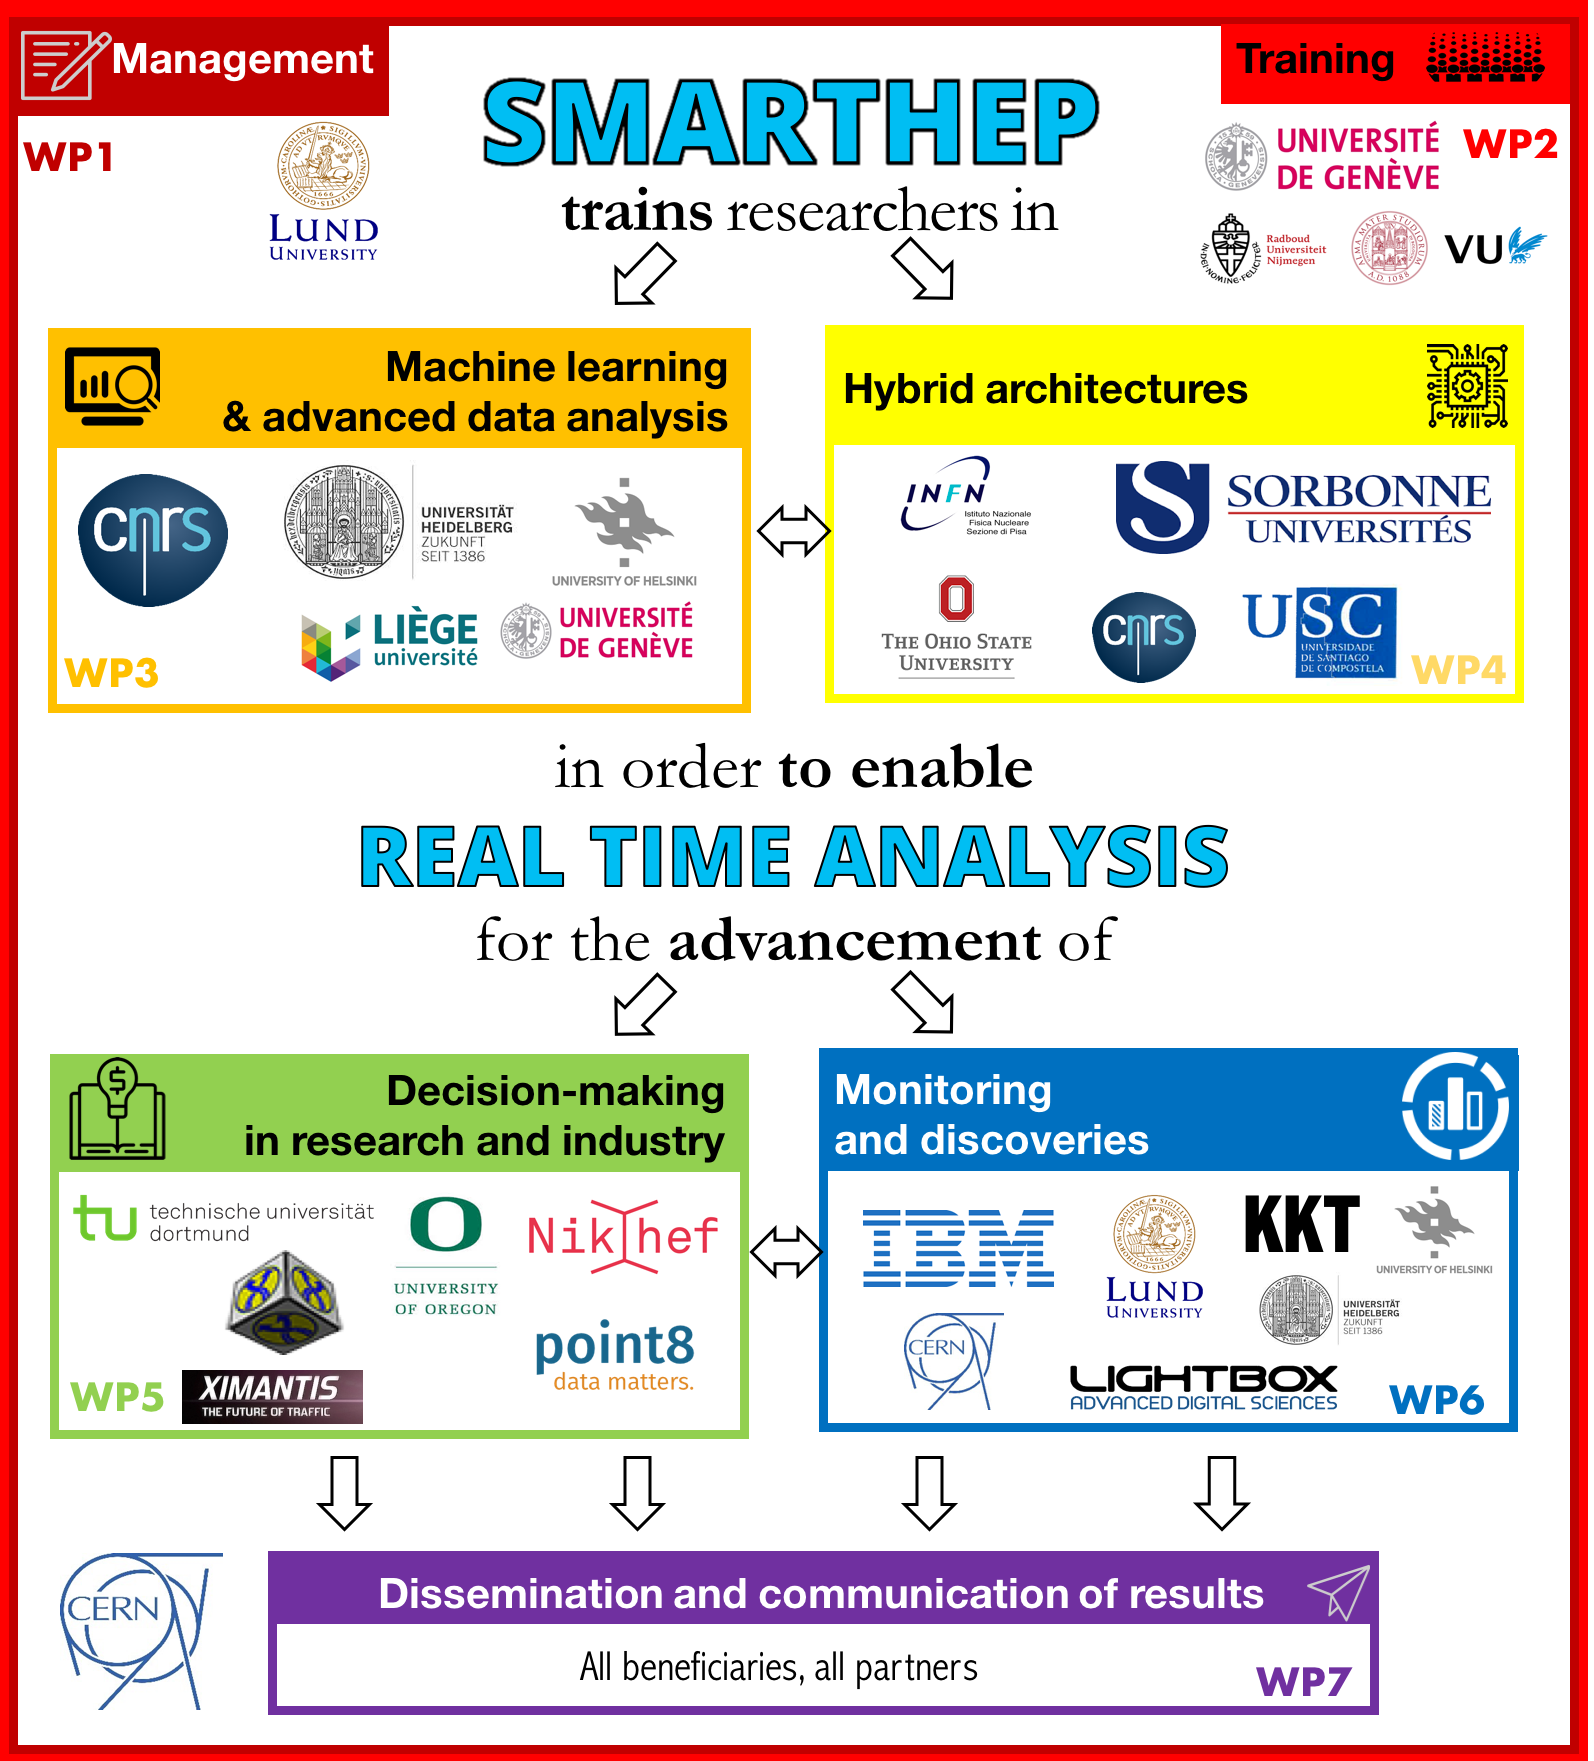
\includegraphics[width=0.9\textwidth]{figs/NetworkCompositionCombinedImplementation.png} %scienceStructure_2.pdf}
%%    \vspace{-8mm} 
%\caption{\acronym implementation strategy and main node expertise.}%\label{fig:implementation}}
%\label{fig:scienceStructure}
%%    \vspace{-3mm} 
%\end{figure}
%\clearpage

%{\color{blue}{Network topics and objectives}.}
\vskip2pt

% that is becoming necessary.
% for research and industry to both contribute to European growth and competitiveness.

%Each of these topics has two aspects: first,
%the development of novel algorithms, analysis techniques and architecture designs,
%as defined in the ESR projects contributing to the research objectives; second,
%the implementation and documentation of these
%algorithms and techniques in a series of publications and software
%packages which will be accessible beyond the
%specific research projects of \acronym and will form its legacy.  


%Academic examples beyond \acronym include social sciences, astrophysics
%and cosmology, Earth sciences and climatology. 

%\acronym has two applications of IoT: 
%ESR3 will focus on a specific type of production chain with the goal
%of improving real-time data analysis and forecast by means of machine
%learning (ML) techniques. ESR7 will also, as secondment at
%WildTreeTech, use similar techniques to consult companies to exploit
%the data collected by their sensors. 
%Due to their architecture, the sensors can produce
%errors, therefore the raw data must be first corrected (filtered
%out). The real-time error correction and data analysis must be
%performed directly on the corresponding microcontrollers or
%single-board computers and due to their limited computational power
%should be highly optimized. 
% The data acquired in real-time by the connected sensors are of
% different nature, unstructured and complex, such as: parts vibration
% data, lubricant and fuel quality, wear particle data, temperature
% measurements, ultrasonic noise detection and flow, infrared
% thermorgraphy, electrical monitoring, etc. These data need to be
% collected, cleaned, aggregated and analyzed in real-time using both
% complex event processing infrastructure and statistical analysis
% techniques.

%%\paragraph{Text from Lightbox, to be reduced to a couple of sentences}
%\textbf{Internet of Things (IoT)} refers to the use of sensors and other
%Internet-connected devices to track and control physical objects
%through the industrial production chain and their subsequent end-user
%delivery steps. 
%In particular the deployment of sensors and systems that are connected
%and can exchange information allows companies to acquire real-time
%information of the operational status of each critical component in an
%industrial production chain. 
%Through IoT, companies may monitor the machine status and performance
%continuously and schedule maintenance only when necessary. 
%
%The combination of real-time and historical measurements data is used
%to infer when the production chain is getting close to a critical
%status that may require actions and to predict when a specific part of
%a machine will have to be fixed or replaced. The adoption of these
%techniques, called 

% Given the heterogeneity of the sensor data,
% ML techniques are beneficial in forecasting when machinery parts need
% intervention or should be replaced. 
%\vspace{1cm}

%\paragraph{Text from Cathi, is reduced, to be placed}
%CATHIS simulator is an interactive system based on software- and
%hardware-modules that provide realistic behaviour (visual and haptic)
%of medical instruments during the training process. 
%The core of the hardware modules is a set of sensors that generate different types of
%raw data (movement, pressure, reaction forces etc.) that must be
%analyzed in real-time and transferred to the software modules for
%further processing. The real-time error correction and data analysis must be
%performed directly on the corresponding microcontrollers or
%single-board computers and due to their limited computational power
%should be 
%highly optimized to fit the limited ressources.

\noindent{\color{blue}{Composition of the network}.} 
%The consortium created for \acronym and includes three major European research institutes, 
%NIKHEF - NL
%CNRS - F
%CERN - SWI
%five universities, 
%Helsinki - FIN
%Lund - SWE
%Dortmund - DE
%Heidelberg - DE
%UniGe - SWI
%and two companies as beneficiaries, 
%IBM - F
%KKT - IT
%as well as seven universities and 
%Oregon - US
%OSU - US
%Pisa - ITA
%Santiago - S
%Radboud - NL
%Paris - FR 
%Amsterdam - NL
%three companies as partners. 
%Ximantis - SWE
%Point8 - DE
%%Lightbox - I

From studies of charm or strange hadrons at LHCb10 to those of light new particles decaying to multi-jet final states at ATLAS and CMS11 to the investigation of processes in collective particle behavior in ALICE, it is now clear that almost every collision at the LHC contains processes which can shed light on fundamental questions in physics. 

Recording this vast amount of data for further processing is not the standard LHC paradigm due to the economic and technological realities of storage costs. 


%%%%%%%%%%%%%%%%%%%%% AB: END HERE %%%%%%%%%%%%%%%%%%%%%%%%

\subsubsection{Research methodology and approach.}
\label{sec:metho}

%MLD: Found this confusing that it says 'four research WPs' but the table shows 7 (and the 7 is only explained later)
%Orig \acronym defines four research WPs in the Table below and Fig.2, each corresponding to a research topic with its specific research objectives. 
%Orig The following table describes the motivations for each of the \acronym research topics and WPs and related ESRs. 
%Orig Additionally, WPs are defined for the management of the consortium, for training, and for outreach and dissemination.  
%Orig A description of the overall tasks for all WPs can be found in Sec.~\ref{sec:WPdescription}. 

\acronym defines four research WPs, corresponding to the research topics listed above, and three WPs for the management of the consortium, for training, and for outreach and dissemination. These are summarized in the Table below and a description of the overall tasks can be found in Sec.~\ref{sec:WPdescription}. Fig 2. gives a schematic view of the four research WPs. 

% MLD I would suggest to stream line what is in the table and add any bigger motivations to the text itself. 

\vskip10pt
\begin{center}
\scriptsize
\resizebox {\textwidth }{!}{%
%\begin{tabular}{@{}p{5mm}p{40mm}p{25mm}p{22mm}p{22mm}p{12mm}p{12mm}p{12mm}}
\begin{tabular}{p{7mm}p{30mm}p{35mm}p{5mm}p{5mm}p{35mm}p{17mm}p{17mm}}
%\begin{tabular}{l|l|l|l|l|l|l|l|}
\toprule
\pbox{8cm}{WP No.} &
\pbox{8cm}{WP Title} &
%This is the number of the beneficiary in the original order
\pbox{8cm}{\Tstrut No. of lead\\Beneficiary\Bstrut} &   
\pbox{8cm}{Start\\Month} &  
\pbox{8cm}{End\\Month} & 
\pbox{8cm}{Activity Type} & 
\pbox{8cm}{\Tstrut Lead Beneficiary\\Short Name\Bstrut} &  
\pbox{8cm}{ESRs\\Involvem't}\tabularnewline\toprule

\cellcolor{red!70!black} \textbf{\color{white}WP1\color{black}}  & Management & Doglioni  & 1 & 48 & Management & \lundentity & - \tabularnewline\hline\midrule

\cellcolor{red} \textbf{\color{white}WP2\color{black}}    & Training   & Sfyrla  & 5 & 42 & Recruitment and training & \unigeentity & All \tabularnewline\hline\midrule

\cellcolor{orange} \textbf{\color{black}WP3\color{black}}   & Data analysis and ML & Gligorov & 1 & 48 & Research& \cnrs & All \tabularnewline \hline%: Software and algorithms enabling RTA
\multicolumn{8}{p{\textwidth}}{
%\textbf{Motivation:} In order to optimize real-time analyses and selections, it is important to employ the most powerful selection algorithms. One of the ML specialties is to find interesting features of data without being explicitly told what to look for. 
%This goal is achieved by minimizing some measure of error in predictions the machine learning algorithm makes. 
%In general, this is an iterative process in which the prediction is altered and the measure of error
%in prediction reevaluated in turn, lowering the total error. 
%The ability to go through a large amount of data and learn non-linear relations between the input
%variables 
%This leads to remarkable performance in tasks of regression and classification.
%The ability to learn from the analyzed datasets also makes ML a very attractive tool towards RTA applications.
%for fast and efficient data analysis
%, since once a decision is made then the data is lost.
Different ML algorithms are investigated by ESRs 1-3, 6, 9 for object reconstruction and feature identification, and for benchmarking and optimisation purposes for ESRs 4, 5, 7, 8, 10-12. 
Custom algorithms for real-time object reconstruction will be deployed by ESRs 3-5, 7, 14, 15.} \tabularnewline \hline \midrule
\cellcolor{yellow} \textbf{\color{black}WP4\color{black}}    & Hybrid architectures & Lacassagne & 1 & 48 & Research & \sorbonneentity  & 3, 4, 8, 9, 11, 15 \tabularnewline \hline % : Novel hardware for detectors and computing 
\multicolumn{8}{p{\textwidth}}{
%\textbf{Motivation:} 
%Innovative solution in hybrid hardware/software architectures are needed for faster, more efficient real-time data analysis, as the complexity and rate of the LHC data does not allow standard processors or data analysis techniques to be competitive (see J.P. Vlimant, \href{https://erez.weizmann.ac.il/pls/htmldb/f?p=101:58:::NO:RP:P58_CODE,P58_FILE:5393,Y}{Machine Learning in Charged Particle Tracking}, Hammers and Nails ML\&HEP Conference, 2017). 

The implementation of ML and detector reconstruction algorithms will be tested on GPUs by ESRs 3, 9, 10 and 11. 
The ATLAS Fast TracKer (FTK) (see ATLAS Collaboration,\href{https://inspirehep.net/record/1614024/}{The ATLAS Fast TracKer}, CERN Document Server, 2016), a hardware solution to particle track reconstruction will be the focus of ESRs 4, 8 and 15. ESR10 will optimize data formats and processing techniques to enable CPUs, GPUs, FPGAs, and hybrids to work together to solve problems which none of these technologies could solve on their own. ESR4 and ESR8 will investigate parallelization and multithreading of current algorithms.
} \tabularnewline \hline \midrule

\cellcolor{lime} \textbf{\color{black}WP5\color{black}}   & Physics applications & Christiansen, Dunford, Voutilainen, Albrecht  & 1 & 48 & Research & \helsinkientity & 1-8, 10-15 \tabularnewline\hline %: Physics measurements and searches
\multicolumn{8}{p{\textwidth}}{
\textbf{Motivation:} 
Physics phenomena beyond the SM are needed to explain many observed phenomena, for example, the existence of massive "dark" matter.%, or 
%%New Higgs searches
%the apparent difference between the measured mass of the recently discovered Higgs boson 
%and what theorized within the SM. %% PS I just removed the clause with Higgs mass, as it is dodgy
ESRs 1-4, 8, 13 and 15 search for new phenomena that could resolve these issues, and measure the properties of the Higgs boson. 
%%LFU
ESRs 5-7 and 10-12 probe the SM prediction that the weak force couplings to all lepton types are equal (Lepton Flavor Universality, or LFU), and that the overall number of leptons of a given type does not change in interactions (Lepton Flavor Violation, LFV). 
%loop-level 
%(CITE RK,RK*), 
%Two researches in this proposal are leading
%ERC research groups to further investigate this question. 
%CD this is best in the quality of the supervision
%%ALICE
The collective behavior of particles measured by ESR15 sheds light on the state of matter present in the early universe a few milliseconds after the Big Bang. 
The common denominator of all those searches and measurements is that they would not be possible without specifically designed data taking techniques with a strong real-time component.
%as detailed in Sec.~\ref{sub:Originality}. 
%\vspace{-2mm}
} \tabularnewline \hline\midrule
%

%To split in 2 tables
%\bottomrule
%%\caption{Work-Package list.}\label{tab:WP}
%\end{tabular}
%}%end of resizebox
%\end{center}
%
%\vskip10pt
%\begin{center}
%\scriptsize
%\resizebox {\textwidth }{!}{%
%%\begin{tabular}{@{}p{5mm}p{40mm}p{25mm}p{22mm}p{22mm}p{12mm}p{12mm}p{12mm}}
%\begin{tabular}{p{7mm}p{30mm}p{35mm}p{5mm}p{5mm}p{35mm}p{17mm}p{17mm}}
%%\begin{tabular}{l|l|l|l|l|l|l|l|}
%\toprule
%\pbox{8cm}{WP No.} &
%\pbox{8cm}{WP Title} &
%%This is the number of the beneficiary in the original order
%\pbox{8cm}{\Tstrut No. of lead\\Beneficiary\Bstrut} &   
%\pbox{8cm}{Start\\Month} &  
%\pbox{8cm}{End\\Month} & 
%\pbox{8cm}{Activity Type} & 
%\pbox{8cm}{\Tstrut Lead Beneficiary\\Short Name\Bstrut} &  
%\pbox{8cm}{ESRs\\Involvem't}\tabularnewline\toprule
%
%%
\cellcolor{green} \textbf{\color{black}WP6\color{black}}   & Industrial applications & Meric, Starovoitov  & 1 & 48 & Research& \dqentity, \heidelbergentity & 1-4, 7-9, 11, 13, 15 \tabularnewline\hline %: Exploitation of RTA 
\multicolumn{8}{p{\textwidth}}{
\textbf{Motivation:} 
Real-time analysis techniques are employed in a variety of industrial contexts.
\acronym selected the cases with the best fit to the physics research program and techniques employed by each ESRs for their industrial secondments.
Most ESRs include a project with concrete industrial deliverables, concerning real-time traffic prediction (ESR1), in-vehicle mobile pattern recognition (ESR2), Internet-of-Things sensors (ESR3, ESR13, ESR15), task optimization and parallelization (ESR4, ESR8), efficient handling of computing clusters (ESR7), medical applications and insurance (ESR9, ESR11).
} \tabularnewline \hline\midrule
%

\cellcolor{cyan} \textbf{\color{black}WP7\color{black}}  & Dissemination, outreach  & Petersen & 1 & 48 & \pbox{8cm}{Dissemination and outreach} & \cern & All \tabularnewline
\bottomrule
%\caption{Work-Package list.}\label{tab:WP}
\end{tabular}
}%end of resizebox
\end{center}
%\vspace{-5mm}
%\end{table}
%\FloatBarrier
%\vspace{-5mm}
%{\color{blue}{Involvement of ESRs in WP and ROs}.}

%\textbf{\acronym answers the question: how do we build detectors which learn from their own performance
%and configure themselves to achieve an optimal understanding of the data which they collect, with as few human assumptions
%as possible, and within the constraints of real-time data processing?} 


%MLD repeative and just a filler
%Our research methodology seeks to apply RTA to novel problems posed by HEP; in turn, the methods employed will evolve from exposure to these new challenges and will be applied to novel industrial and commercial problems.
%This methodology is made explicit in Fig. 1.%~\ref{fig:scienceStructure}. 

%Each ESR develops novel methods in light of HEP problems, and applying DS methods to commercial applications. 
%This ensures that ESRs will be fully immersed in both HEP, while, at the same time, 
%advancing the state of the art in industry. 
%, 
%figure below. 
%\begin{center}
%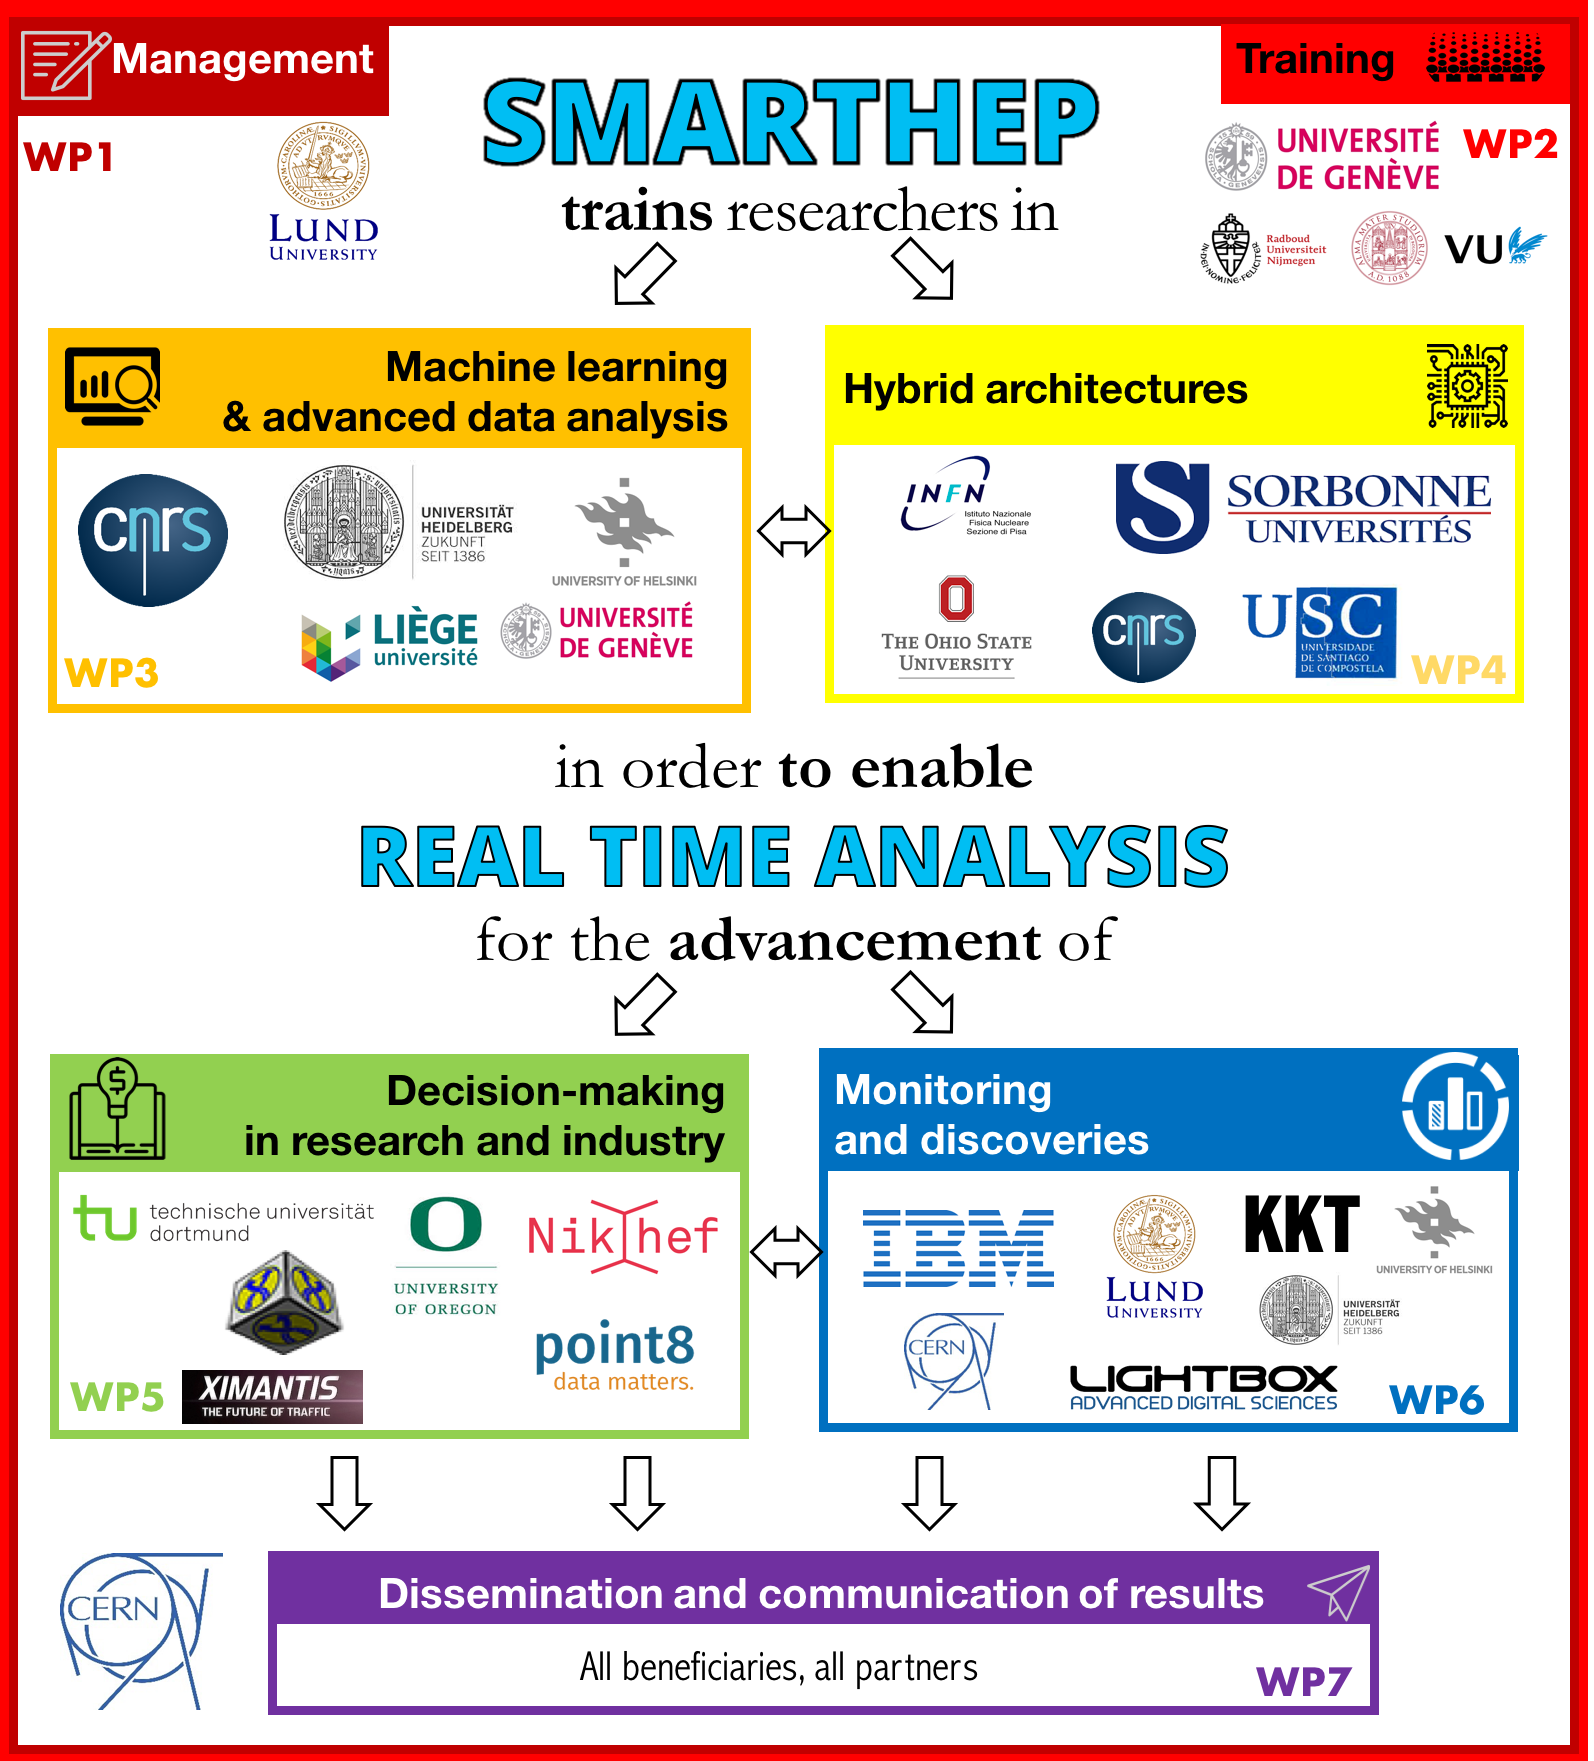
\includegraphics[width=0.75\textwidth]{figs/NetworkCompositionCombinedImplementation.png}\\ %scienceStructure_2.pdf}
%\end{center}

%This is in the figure now 
%%CD: I think a 2-column list here is unnecessary if you massage the endings of the sentences a bit, but you can change it back
%\vspace{-2mm}
%\begin{multicols}{2}[]
%\small
%\begin{enumerate}%{\leftmargin=1em}
%    \item Identify dataset to be studied, and key features/variables to be analyzed, clearly define intermediate milestones and research~path;
%    \item Research and master techniques to be applied to the dataset employed;
%    \item For commercial products, in collaboration with industrial partners: research market aspects and plan how to create value;
%    \item Implement identified techniques using appropriate computing infrastructures (local computing clusters, distributed LHC computing grid, hybrid architectures, etc.);
%    \item Present progress of each deliverable regularly within \acronym, group meetings, conferences. Actively seek feedback for improvement,
%     as described in Sec.~\ref{sub:progressMonitoring};
%    \item On completion, follow up on applications and external feedback on deliverables. 
%\end{enumerate} 
%\end{multicols}
%\vspace{-2mm}
%\vskip 5mm
%


%\vskip5pt
%and Network resources are shared to allow for their optimal completion.

%%%REPETITION ALARM: why do we have to have two tables? 

%(For ETN, it should be explained how the individual projects of the recruited researchers will be integrated into ? and contribute to 
% the overall research program. EJD and EID proposals should describe the research projects in the context of a doctoral training program)

%The action should be divided in Work Packages and described in the table below. The Work Packages should reflect the research objectives. Only brief headings and overviews of the Work Packages should be presented in Table 1.1. More details in terms of actual implementation should be provided in the tables under section 3.1.
 
%\FloatBarrier
%\begin{table}[!htb]
\vspace{-2mm}
\subsubsection{Originality and innovative aspects of the research program} 
\label{sub:Originality}
%((in light of the current state of the art and existing programs / networks / doctoral research trainings)

HEP experiments are by their very nature built around \textbf{training}, as around a third of all LHC collaborations consist of PhD students.
This combination of a collaborative, training-based research culture, and a focus cutting-edge technologies using the largest datasets produced make \acronym an ideal and unique training program.

%\begin{wrapfigure}{r}{0.75\textwidth}
%	\vspace{-5mm}
\begin{center}
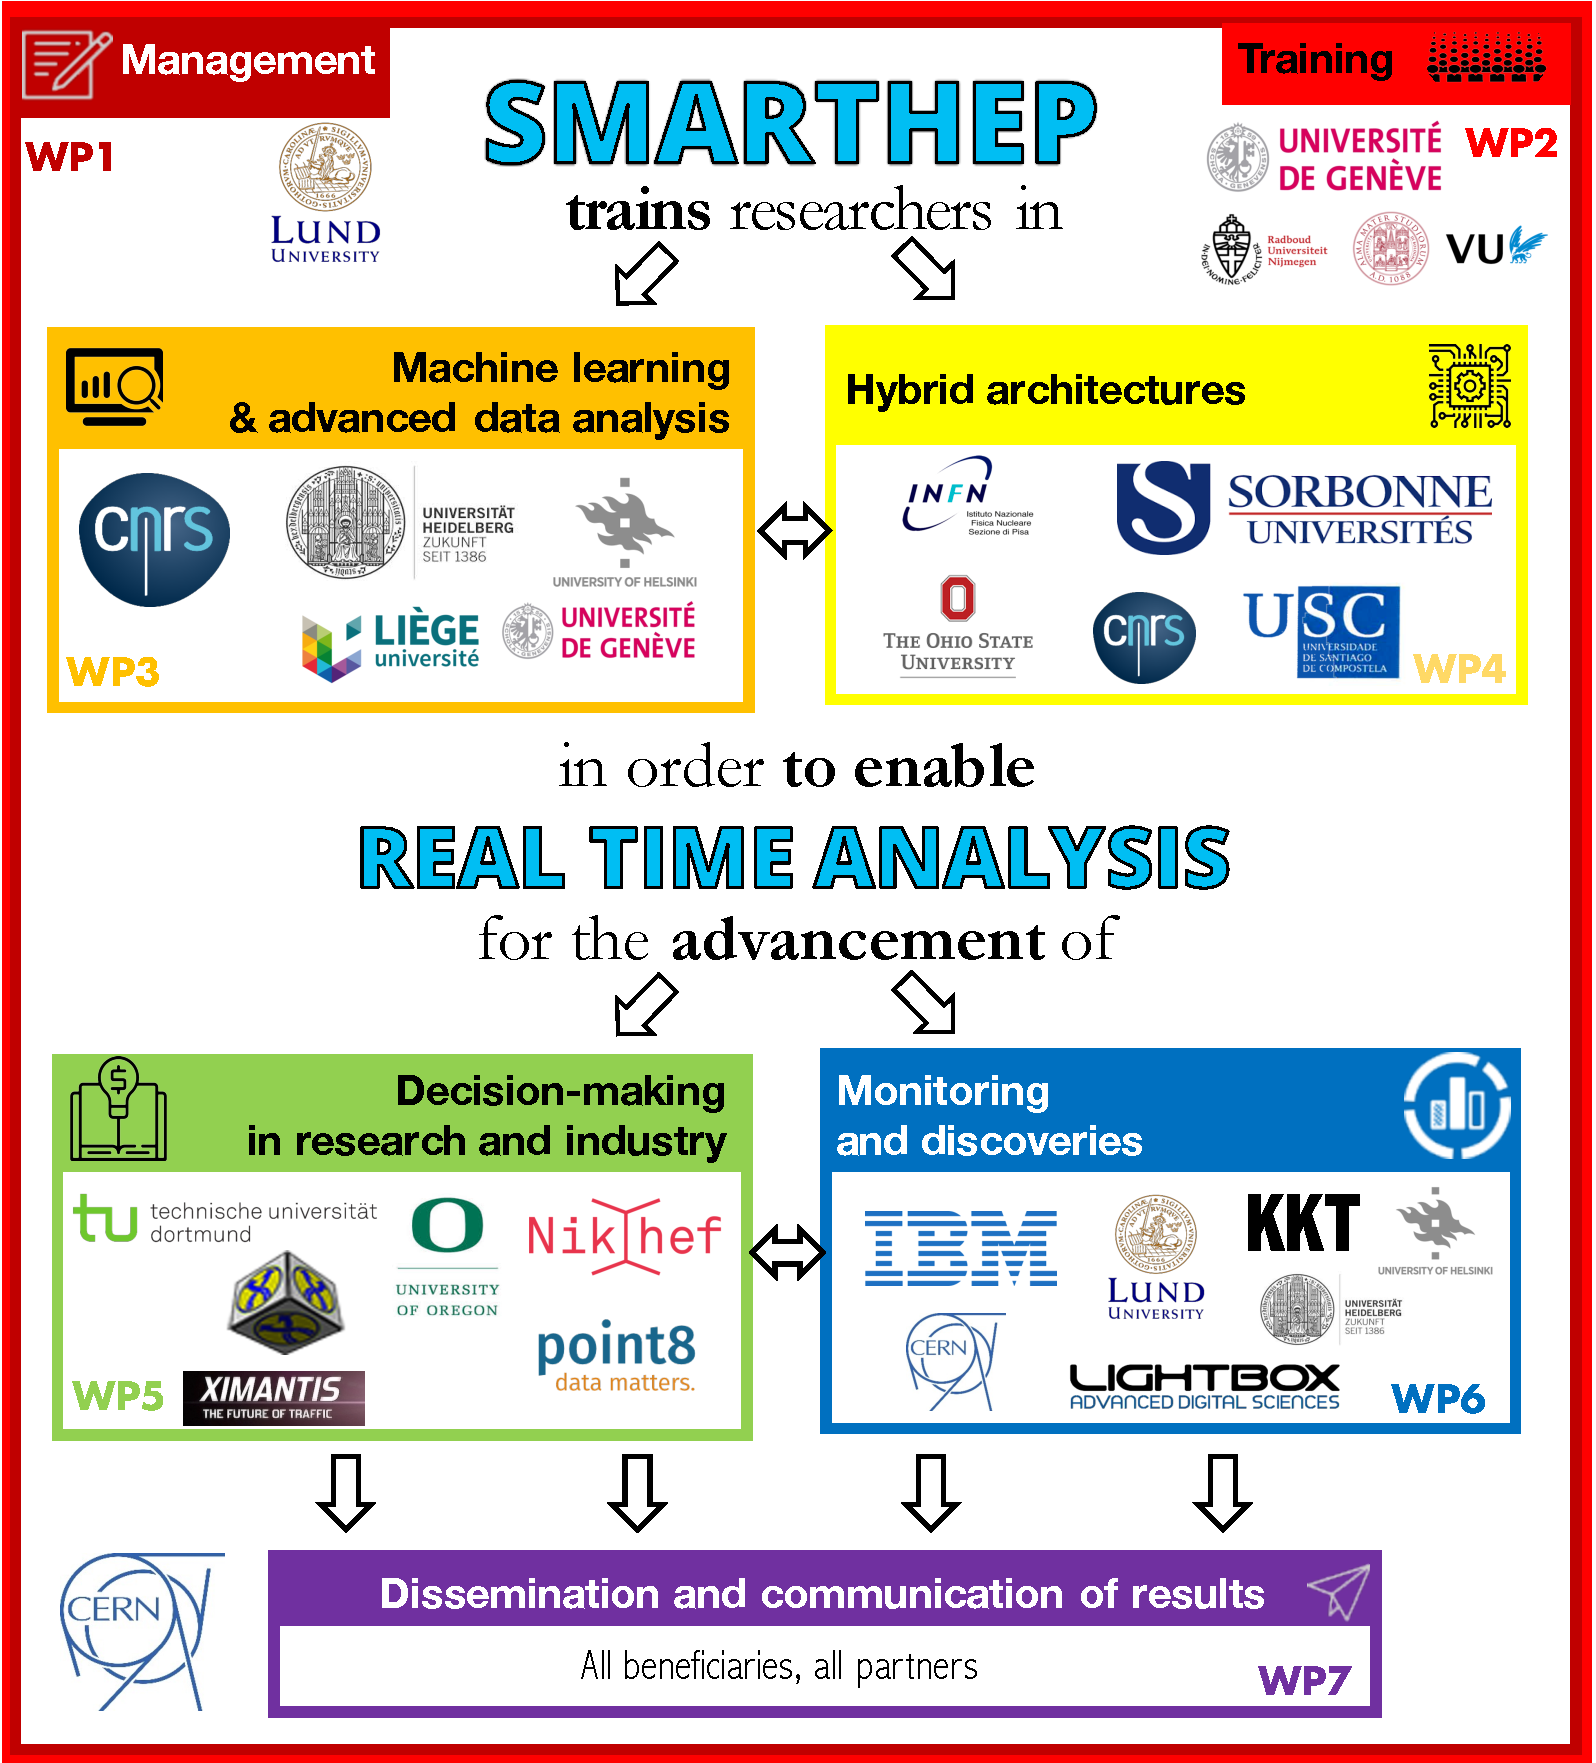
\includegraphics[width=0.7\textwidth]{figs/NetworkCompositionCombinedImplementation} %scienceStructure_2.pdf}
    %\vspace{-8mm} 
%\label{fig:scienceStructure}
%    \vspace{-3mm} 
\begin{center}\footnotesize \label{fig:implementation}
Figure 1: \acronym implementation strategy and main node expertise.
\end{center}%\label{fig:implementation}}
\normalsize 
\vspace{-2mm}
\end{center}
 
\noindent {\color{blue}{1. Researchers from \acronym learn to process large datasets using novel analysis techniques}.}
%  \begin{wrapfigure}{r}{0.7\textwidth}
%%\begin{figure}{l}{\textwidth}
	%\vspace{12mm}
%	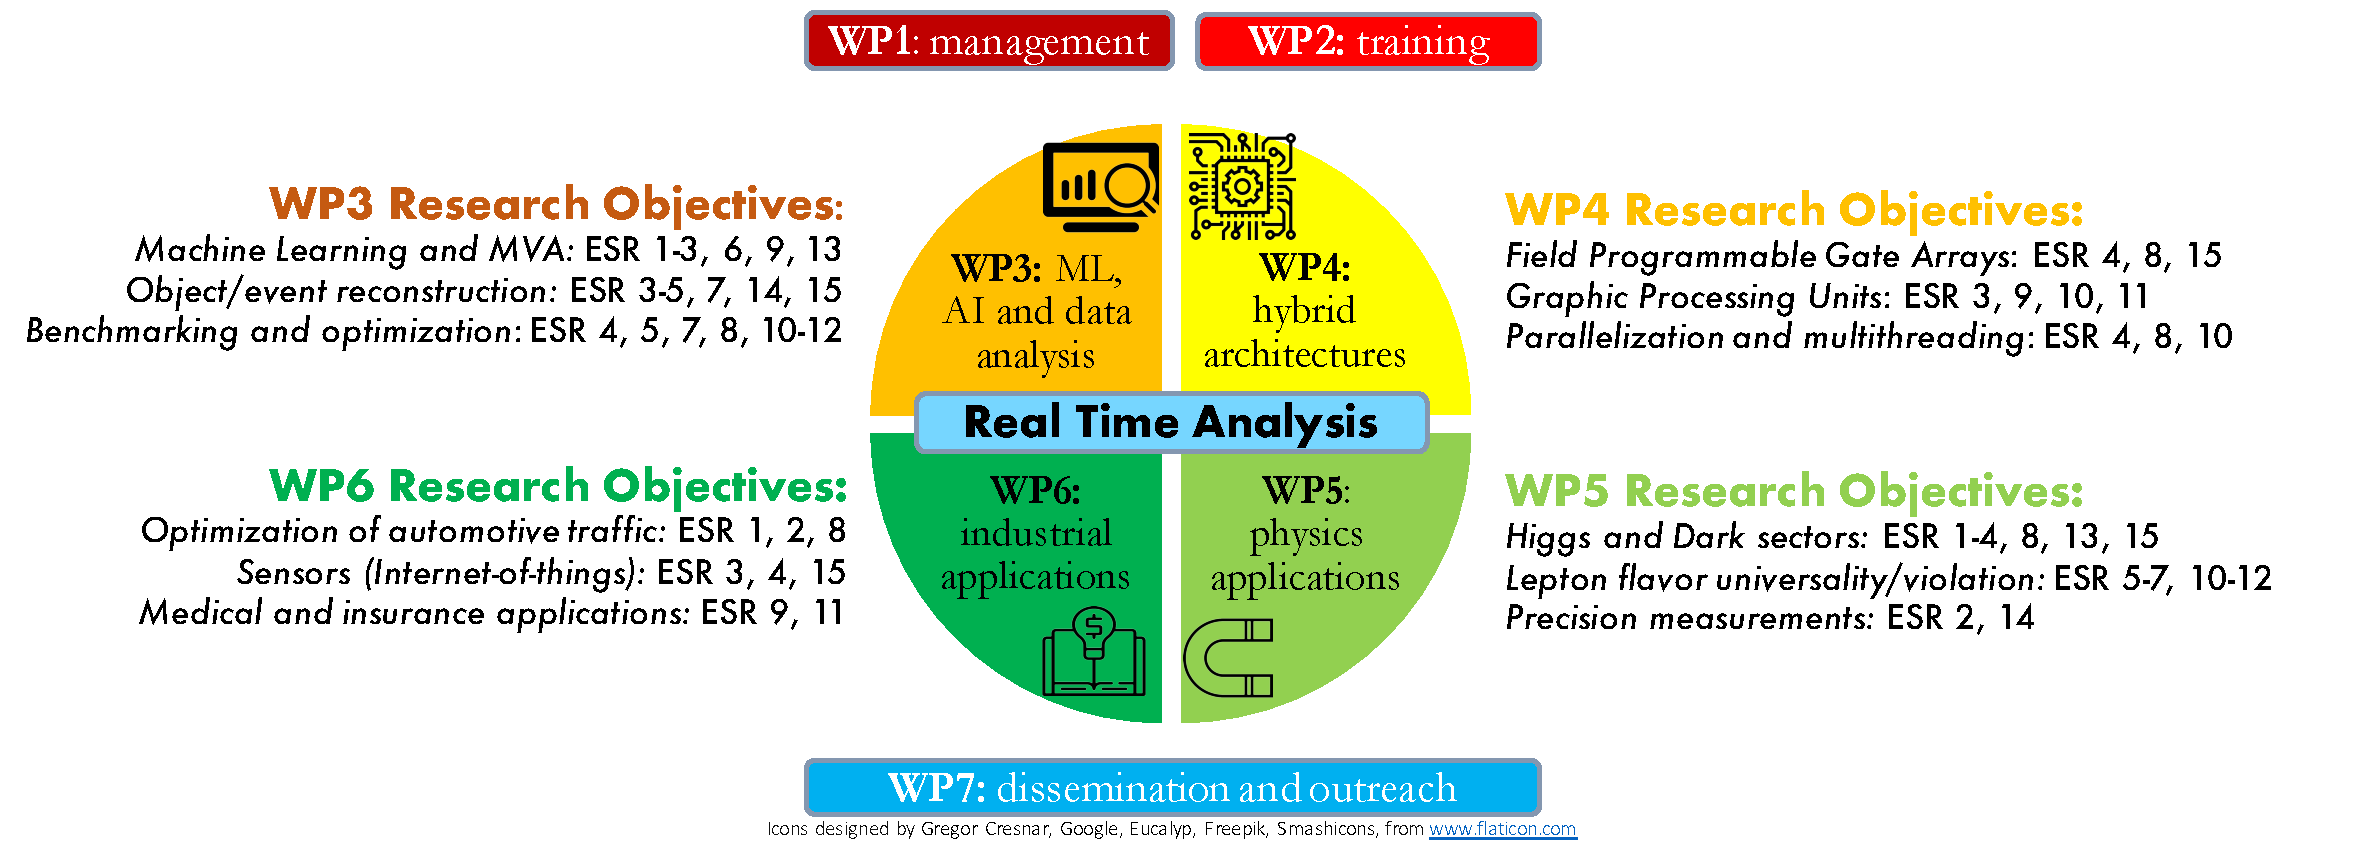
\includegraphics[width=0.7\textwidth]{figs/WPs} %scienceStructure_2.pdf}
%    \vspace{-5mm} 
%	\caption*{Figure 2 : Structure and Research Objectives of the Work Packages.\label{fig:WPs}}
     %\vspace{-5mm} 
%%\begin{figure}	
%\end{wrapfigure}
A large part of the novelty of this proposal is the volume of data which will be processed, comparable to the largest commercial tasks. 
% MLD this is a great sentence but it is just out of place here
%This is true across both academic and non-academic applications:
%an estimated 90$\%$ of generated data is considered too expensive to store\footnote{\href{http://www.mckinsey.com/insights/business_technology/big_data_the_next_frontier_for_innovation}{2010 report on Big Data by McKinsey\&Company.}}.
One can compare Facebook and e.g. the LHCb collaboration.
%MLD I switched to numbers because then the comparison is more powerful (also shorter!)
The former processes $O(100)$ petabytes of data per year and spends 500M dollars a year on computing\footnote{Facebook, \href{http://www.datacenterknowledge.com/the-facebook-data-center-faq-page-three/}{The Facebook Data Center FAQ}, 2010.} while the latter processes  $O(1000)$ petabytes of data per year and spends around 7M dollars a year on computing\footnote{Private communication, \href{mailto:peter.clarke@ed.ac.uk}{Prof. Peter Clarke}, University of Edinburgh.}.
The essential difference is that Facebook stores and distributes this data to its users while LHC experiments largely process and then dispose of the data.
%MLD I felt this was not needed to make the above argument. It removes your figure 3 but see my comment from the email. 
%An example of this are the physics searches and measurements performed solely using trigger information.
%In these searches only a small fraction of each event, regardless of whether LHC experiments are able to record it for offline reconstruction or not, is saved for further processing. 
%This overcomes the storage limitations and allows to be more than an order of magnitude more sensitive to certain new particles (e.g. associated to Dark Matter, as in Fig.3).

To achieve and go beyond this, the LHC experiments need a more systematic application of RTA, machine learning and hybrid architectures for HEP. Examples are methods using Deep Learning techniques, which build high-level features from raw data (ESR1 and ESR2), using Recurrent Neural Networks (RNNs), which learn ordered patterns in the data and can be applicable both to tracking and to model paths taken by vehicles (ESR10), and Generative Adversarial Networks (GAN) for anomaly detection techniques (ESR13).
This paradigm shift can be used in industry as well, while the research environment can benefit from a generation of ESRs trained in industrial grade algorithms and tools. 

%\begin{wrapfigure}{r}{0.4\textwidth}
%	\vspace{-4mm}
%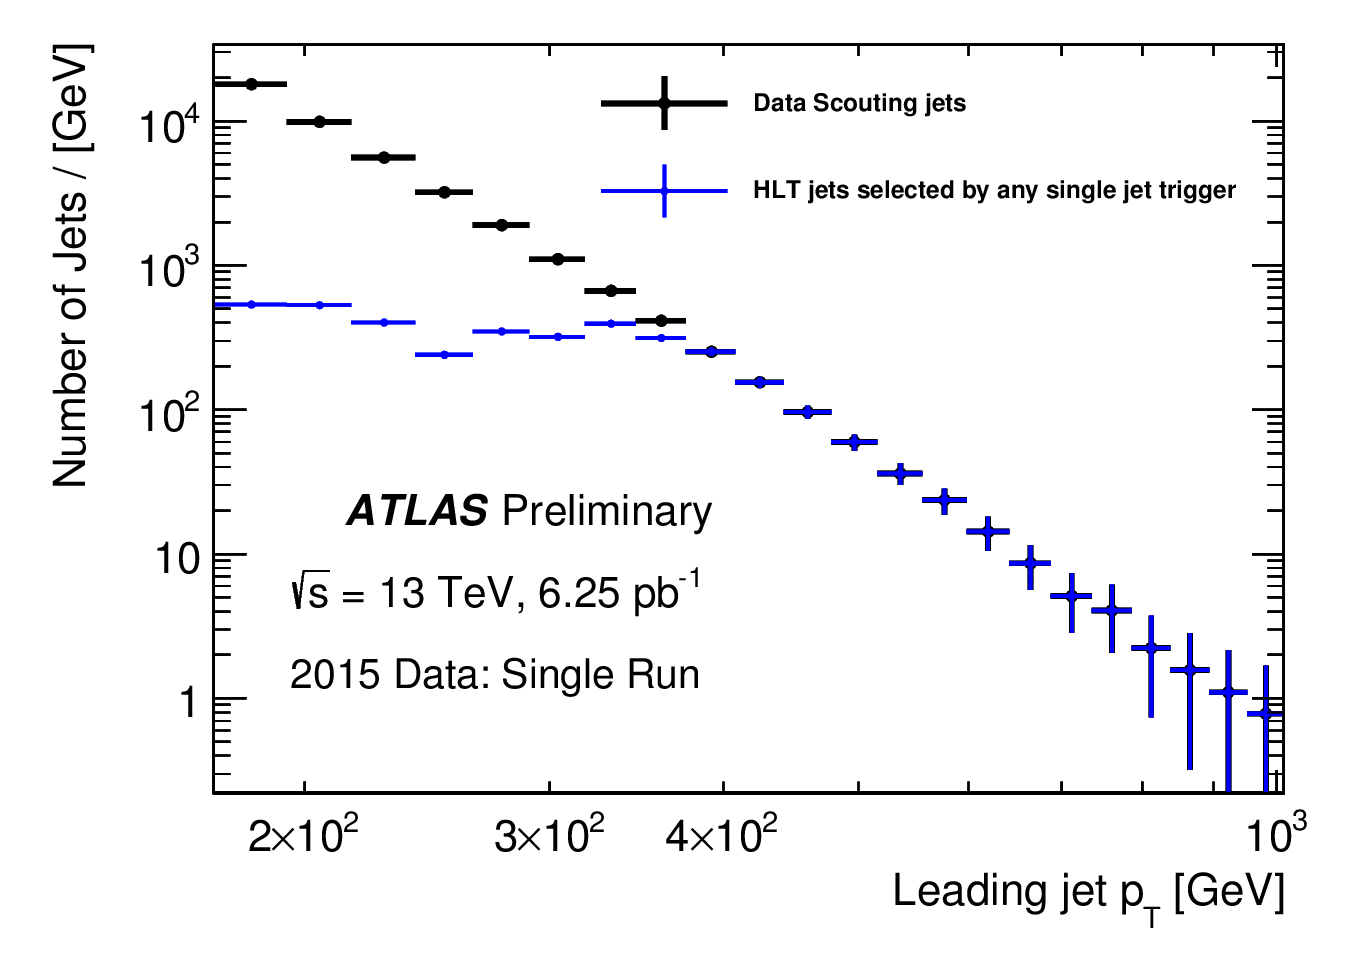
\includegraphics[width=0.4\textwidth]{figs/TLA.png} 
%    \vspace{-10mm} 
%    \caption*{Figure 3: Example of the number of events using traditional techniques (blue) compared to a trigger-level analysis (black)
%in the search for new particles. Main analyzers: Boveia, Doglioni, Starovoitov, Dunford. \label{fig:TLA}}
%\vspace{-4mm}
%    \end{wrapfigure}
%    \vspace{-3mm} 
%Real-time analysis, machine learning and hybrid architectures have so far not been systematically
%applied to HEP problems. 
%Moreover, even where toolkits exist for HEP,
%notably \tmva\ or \scikit\, they are little more than a collection
%of individual algorithms applied in an ad-hoc manner.
%The research program of \acronym is developed coherently around 
%four main research questions that are at the forefront of 
%the long-term goals of all major LHC experiments. 
%which work against each other, 
%one generating examples and the other classifying them. 
%The classifying network gets a normal score, while 
%the generating network is scored when it can create an example	
%that escapes the classifier, so to make the classifier more 
%sensitive to non-standard cases as it is essential in RTA
%where rare, non-standard but interesting events risk being lost for good. 

%%CD: possible text about machine learning
%An additional driving challenge for the \acronym research program is the continuous need for improvement of background rejection
%techniques once the data has been taken. The discovery of the Higgs boson in 2012, which lead to the award of a Nobel Prize in Physics, has 
%opened the door to a whole new set of measurements of the properties of this new particle and possible discoveries 
%of deviations from the Standard Model. However, the frequency with which
%the Higgs boson particle is produced is minuscule compared to the rates of the backgrounds yielding the same detector signatures as the Higgs boson.  
%An efficient background rejection is key for both measurements involving the Higgs boson and similarly rare particles. 
%The need for novel techniques that only select the interesting events and reject the background is acute, in high energy physics and in
%commercial applications alike. The first challenge of analyzing events in real-time addressed by \acronym also has similar needs: 
%the current paradigm of triggering on simple features 
%ignores the growing importance of the analysis of raw, unstructured, data across both academia
%and industry. For both issues, a series of techniques known as machine learning, multivariate analysis, and 

\noindent {\color{blue}{2. The \acronym program of searches and measurement could lead to breakthroughs in our understanding of nature}}
Research topics chosen to drive conceptual developments within \acronym have potential to lead to the discovery of new physics beyond the Standard Model, but only RTA techniques enable full exploitation of the LHC dataset. 
%the full statistical reach of the LHC data to be exploited. 
%Only RTA techniques will enable such discoveries. 
ESRs working on physics topics will target common challenges, e.g. when real-time algorithms and reconstruction techniques are not sufficiently advanced to distinguish signal from noise, or when the statistical power of the dataset is not fully exploited if objects are reconstructed with traditional techniques. 
%The advanced tools under design in \acronym
%will allow the real-time systems of LHC 
%experiments to improve coherently. 

% MLD this sudden detailed motivation of the physics seems out of place. This section is supposed to be motivating why the training program is unique. Also the level of detail here is not consistent with other parts. 
Examples include studies of lepton flavor and its conservation and universality in different final states and experiments (ESR 5-7, 9, 11-12), and dark matter mediators and new light particles\footnote{M. Chala et al, \href{http://arxiv.org/abs/1503.05916}{Constraining Dark Sectors with Monojets and Dijets}, JHEP 1507 (2015) 089.}.
The volume of data needed to be sensitive to these rare processes is the perfect testing ground for improved real-time techniques for ESR1 and 8.  
RTAs looking for dark matter mediators in ESR13 and 15, and the search for new particles of ESR3 and 4 using ML have never been performed at the LHC, nor have generic searches for rare new phenomena as in ESR2.
Measurements in ESR2 and 15 precisely probe the SM in the Higgs and heavy ions sectors. 

The choice of physics topics that all need RTA to achieve beyond-state-of-the-art results ensures advancement in detector development and contribution to major advances in key analyses of LHC data.
%paving the way to understand the main questions of our universe. 

\noindent {\color{blue}{3. ESRs in \acronym deploy and disseminate their research at a unique time for particle physics}.}
As highlighted by the HEP Software Foundation Whitepaper$^{4}$, the period 2019-2023 is ideal for this R\&D in HEP, as it is a time of transition between LHC data taking periods that will be necessary to prepare for an upgrade of the LHC accelerator where the amount of data delivered will make RTA techniques  the key to pursue the physics programs of the four main LHC experiments.
The systematic optimization of HEP experiments by \acronym will boost the performance of the current and planned upgrades of the CERN based accelerator experiments.
Furthermore, the developed toolkits will be advertised at international conferences and thus the developed methods will shape the online event selection of all future HEP experiments. 

\noindent {\color{blue}{4. \acronym researchers develop techniques and infrastructures that can be exploited in industrial applications, as well as in HEP}.}
The close links of the research institutes of the consortium with the industry partners means that the ESRs will directly drive the development of novel industrial products, while also bringing professional methods of data mining that are exercised in large companies into the academic environment. 
Most modern methods applied in research can in this way be transferred more easily to industry applications in automotive traffic optimization (ESR1-2, 6, 8) and analysis of sensor data for IoT and medical applications (ESR3-4, 9, 11, 13, 15).
%JA: not , 14 (??)) 
The proposed algorithms and the use of ML methods on these scales of data are novel to both HEP and industry. 
By exposing industry-grade methods to the volume and complexity of HEP data, we will stimulate their development in a complementary way for the benefit of industry.

%\noindent {\color{blue}{5. \acronym researchers share information and write sustainable code}.}
%As the \acronym WPs intimately depend on each other,
%we will make the sharing of information, methods, and data between ESRs a centrepiece
%of our research strategy. Dedicated computing resources will
%be provided by the LHCb and ATLAS CERN groups for \acronym, and all ESRs will
%be required to 
%maintain and develop their research within this space
%accessible to the whole network. ESRs will be trained in
%maintaining digital logbooks\footnote{For example on \href{https://github.com}%{https://github.com} and using \href{https://jupyter.org}{Jupyter}.}%
%and documentation %so that other members of the network can profit from it, and 
%to ensure that
%they develop \textbf{sustainable} software, reusable both by
%other \acronym ESRs and later by others in
%the community. 
%Developing \textbf{sustainable software} is commonplace in industry but novel
%in physics, where the state of the art is usually a repository with notes about individual commits
%and a Doxygen server giving a web-based overview of the classes in the software. 
%By training the ESRs in state of the art industrial development methods, \acronym will also make a significant
%step forward in the development of physics software.
%Sustainability will encompass both the design (language, definition
%of interfaces and objects) of the software as well
%its documentation (writing individual methods a non-expert can read,
%comment cards in the source code, external documentation explaining algorithms and program flow).
%All developed methods and code will be shared; however, the data of the ALICE, CMS, LHCb and %ATLAS experiments will be treated according to the regulations of the
%respective collaborations. %The collaborative approach which is mandated by
%the described interdependency of the different aspects of our research program is at the heart of our research methodology.